\section{Niezmienniki Wasiljewa}
\index{niezmiennik!Wasiljewa|(}
\label{sec:vassiliev}
% DICTIONARY;invariant, finite type;niezmiennik, skończonego typu
Niezmienniki Wasiljewa (znane także jako niezmienniki skończonego typu) umożliwiają radykalnie nowe podejście do węzłów.
Około 1989 roku odkryli je niezależnie Wiktor Wasiljew, w~oparciu o~teorię osobliwości, oraz Michaił Goussarow, metodami kombinatorycznymi.
% Wasiljew: V. A. Vassiliev, Cohomology of knot spaces, Theory of Singularities and its Applications (ed. V. I. Arnold), Advances in Soviet Math., 1 (1990) 23-69.
My przedstawimy to drugie podejście.
Niezmienniki Wasiljewa najlepiej zrozumieć, jeśli osłabimy trochę definicję węzła i będziemy rozważać także krzywe z~samoprzecięciami.

Uważam, że przyjemnym wprowadzeniem do niezmienników Wasiljewa jest artykuł \cite{chmutov12} Chmutowa.
Za najlepsze uważa się pracę \cite{barnatan_95}: Bar-Natan, jej autor, pozostaje do dziś jedną z~najważniejszych osób dla rozwoju tego działu matematyki.
Oprócz tego jest jeszcze pięknie zilustrowana książka \cite{duzhin12} trzech rosyjskich matematyków, będąca obszernym kompendium wiedzy o~węzłach singularnych. % oraz ciekawy podręcznik \cite{dye16}, który rozwija od podstaw teorię węzłów wirtualnych i~klasycznych równocześnie; węzły wirtualne to coś innego niż singularne, w równoważności dopuszcza się inne ruchy!
Szkielet sekcji oparliśmy natomiast o piętnasty rozdział podręcznika Murasugiego, \cite{murasugi96}.

% DICTIONARY;knot, singular;węzeł, singularny
\begin{definition}[węzeł singularny]
\index{węzeł!singularny}%
    Niech $f \colon S^1 \to \R^3$ będzie kawałkami liniową funkcją, która jest różnowartościowa poza skończenie wieloma punktami.
    Załóżmy dodatkowo, że
    \begin{itemize}
        \item włókna -- przeciwobrazy punktów -- funkcji $f$ są co najwyżej dwuelementowe;
        \item jeżeli dwa różne punkty mają ten sam obraz, to węzeł $K = f(S^1)$ przecina się tam pod kątem prostym.
    \end{itemize}
    Obraz funkcji $f$ nazywamy węzłem singularnym.
\end{definition}

Gdy używamy słowa węzeł, nigdy nie mamy na myśli węzła singularnego.
Punkt, gdzie węzeł singularny tnie samego siebie, nazywamy wierzchołkiem i~oznaczamy pogrubioną kropką na diagramie.
\index{wierzchołek (węzła singularnego)}%
Oto garść przykładów węzłów singularnych:

\begin{comment}
\begin{figure}[H]
    \centering
    \begin{minipage}[b]{.14\linewidth}
        \centering
        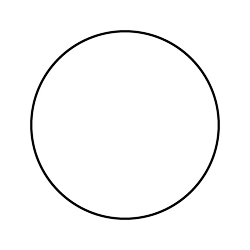
\includegraphics[width=\linewidth]{../data/virtual_0_1.png}
        \subcaption{$0_1$}
    \end{minipage}
    \begin{minipage}[b]{.14\linewidth}
        \centering
        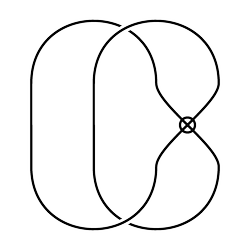
\includegraphics[width=\linewidth]{../data/virtual_2_1.png}
        \subcaption{$2_1$}
    \end{minipage}
    \begin{minipage}[b]{.14\linewidth}
        \centering
        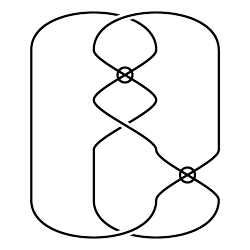
\includegraphics[width=\linewidth]{../data/virtual_3_1.png}
        \subcaption{$3_1$}
    \end{minipage}
    \begin{minipage}[b]{.14\linewidth}
        \centering
        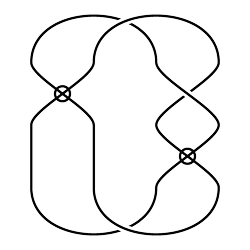
\includegraphics[width=\linewidth]{../data/virtual_3_7.png}
        \subcaption{$3_7$}
    \end{minipage}
    \begin{minipage}[b]{.14\linewidth}
        \centering
        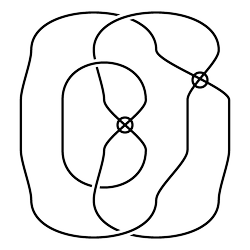
\includegraphics[width=\linewidth]{../data/virtual_4_1.png}
        \subcaption{$4_1$}
    \end{minipage}
    \begin{minipage}[b]{.14\linewidth}
        \centering
        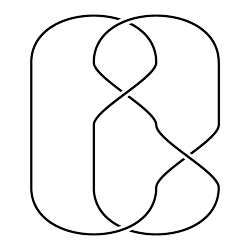
\includegraphics[width=\linewidth]{../data/virtual_4_108.png}
        \subcaption{$4_{108}$}
    \end{minipage}
\end{figure}
\end{comment}

Podamy teraz definicję równoważności dla węzłów singularnych, zupełnie analogicznie do definicji \ref{def:equivalent_knots_2} dla zwykłych węzłów.

\begin{definition}[płaski dysk]
    Niech $A$ będzie wierzchołkiem węzła singularnego $K$, $B_A$ jego małym domkniętym otoczeniem, zaś $P_A$ płaszczyzną, która zawiera $B_A \cap K$, mały fragment węzła wokół wierzchołka.
    Dysk $P_A \cap B_A$ nazywamy płaskim dyskiem wokół wierzchołka $A$.
\end{definition}

\begin{definition}
    Dwa singularne węzły $K, L$ są równoważne, co zapisujemy jako $K = L$, jeśli istnieje zachowujący orientację homeomorfizm $\varphi$ przestrzeni $\R^3$ w~siebie, który przenosi jeden węzeł na drugi: $\varphi(K) = L$ oraz indukuje bijekcję między rodzinami płaskich dysków $K$ i~$L$.
\end{definition}

Ten drugi warunek gwarantuje nam, że skrzyżowania wokół podwójnych punktów nie ulegną zniszczeniu.
Istnieje podobne kryterium dla diagramów, odpowiednik twierdzenia Reidemeistera.

\begin{proposition}
\index{ruchy Reidemeistera}
\index{ruch $\Omega$}
    Dwa singularne diagramy są równoważne dokładnie wtedy, kiedy można między nimi przejść przy użyciu ciągu izotopii otaczających, ruchów Reidemeistera, operacji $\Omega_4$ (dwóch wariantów III ruchu Reidemeistera z wierzchołkiem):
\begin{comment}
    \[
        \VirtualReidemeisterIIIa \cong_{\Omega_{4a}} \VirtualReidemeisterIIIb
        \quad\quad
        \VirtualReidemeisterIIIc \cong_{\Omega_{4e}} \VirtualReidemeisterIIId
    \]
\end{comment}
    oraz zupełnie nowego ruchu $\Omega_5$ przypominającego flype:
\begin{comment}
\[
    \VirtualOmegaVa \cong_{\Omega_{5a}} \VirtualOmegaVb
\]
\end{comment}
\end{proposition}

Uwaga: Murasugi podaje tylko jedną nową operację, wydaje nam się, że wszyscy nie mogą mieć racji.
Ufamy pracy Nelsona, Oyamaguchiego, Sazdanovica \cite{sazdanovic19} gdzie pokazano, że ten zestaw ruchów jest minimalny.

Załóżmy teraz, że mamy jakiś niezmiennik węzłów $v$ o~wymiernych wartościach i~chcemy przedłużyć go do niezmiennika $\hat v$ węzłów singularnych.
Najprościej zrobić to rekurencyjnie.
Niech $\hat v$ będzie już określony dla singularnych węzłów o co najwyżej $n - 1$ wierzchołkach i~wybierzmy dowolny węzeł i diagram o~$n$ wierzchołkach.
Okazuje się, że jeżeli położymy
\begin{comment}
\begin{equation}
    \hat v\left(\SingularCrossing\right) = \hat v\left(\MediumSkeinPlus\right) - \hat v\left(\MediumSkeinMinus\right),
\end{equation}
\end{comment}
to dostaniemy dobrze określoną funkcję: jeżeli $L = K$ jest tym samym węzłem singularnym z~innym diagramem, to $\hat v(L) = \hat v(K)$.

Funkcję $\hat v$ nazywamy niezmiennikiem singularnym indukowanym przez niezmiennik węzłów $v_0$.

\begin{definition}[rząd niezmiennika]
\label{def:vassiliev_order}%
\index{rząd niezmiennika}%
    Niech $v$ będzie niezmiennikiem singularnym.
    Mówimy, że $v$ jest niezmiennikiem Wasiljewa rzędu co najwyżej $n$, jeśli dla dowolnego singularnego węzła $K$ o $n + 1$ wierzchołkach zachodzi $v(K) = 0$.
    Jeśli dodatkowo $v$ nie jest rzędu co najwyżej $n - 1$, to mówimy, że jest rzędu dokładnie $n$.
\end{definition}

Czas na garść przykładów niezmienników skończonego typu oraz niezmienników, które nie są skończonego typu.

\begin{example}
\index{wielomian!Conwaya}%
    Niech $K$ będzie węzłem, zaś $\conway_K(t) = \sum_k \conway_{2k} z^{2k}$ jego wielomianem Conwaya.
    Współczynnik $\conway_{2k}$ indukuje niezmiennik Wasiljewa rzędu dokładnie $2k$.
\end{example}

\begin{proof}
    Jak wspomina Chmutow w \cite{chmutov12}, porównanie relacji kłębiastej dla wielomianu Conwaya z tą dla niezmienników Wasiljewa pokazuje, że wielomian Conwaya singularnego węzła o~$m$ punktach podwójnych jest podzielny przez $z^m$, co dowodzi już, że $c_{2k}$ jest niezmiennikiem rzędu co najwyżej $2k$.

    Bar-Natan w 1991 pokazał, że $\conway_{2k}$ jest niezmiennikiem rzędu dokładnie $2k$.
\end{proof}

\index{hipoteza!Lin-Wanga}%
Lin oraz Wang \cite{wang96} w~1994 roku na podstawie niezmienników małych rzędów, to jest $v_2$ oraz $v_3$, wysunęli następującą hipotezę: istnieje uniwersalna stała $C$ taka, że
\begin{equation}
    |v_k(K)| \le C (\crossing K)^k.
\end{equation}

Hipotezę wkrótce udowodniono, najpierw dla węzłów (Bar-Natan, \cite{barnatan95}), nieco później także dla splotów (Stojmenow, \cite{stoimenow_01}).
Wartość stałej $C$ trudno obliczyć, dlatego Stojmenow zaproponował \cite[problem 1.17]{ohtsuki02} ograniczenie się do przypadku $v_k = \conway_k$.

\begin{conjecture}
    Niech $L$ będzie splotem.
    Wtedy
    \begin{equation}
        |\conway_k(L)| \le \frac{(\crossing L)^k}{2^kk!}.
    \end{equation}
\end{conjecture}

Nierówność jest nietrywialna tylko dla splotu $L$ z~$k+1, k-1, \ldots$ składowymi; trywialna dla $k = 0$, łatwa dla $k=1$ (wtedy $\conway_1$ jest indeksem zaczepienia splotów o~dwóch składowych) oraz udowodniona dla węzłów i~$k=2$ przez Polyaka, Viro w~2001 (\cite{polyak01}).

\begin{example}
\index{wielomian!Jonesa}%
    Niech $\jones_K(t)$ będzie wielomianem Jonesa węzła $K$.
    Dokonajmy podstawienia
    \begin{equation}
        t := e^x = 1 + x + \frac{x^2}{2} + \frac{x^3}{6} + \ldots,
    \end{equation}
    a~następnie rozwińmy wynik w~szereg Taylora:
    \begin{equation}
        \jones_K(e^x) = \sum_{k = 0}^\infty b_k x^k.
    \end{equation}
    Współczynnik $b_{k}$ indukuje niezmiennik Wasiljewa rzędu co najwyżej $k$.
\end{example}

Ten i podobne wyniki dla wielomianów HOMFLY, Kauffmana uzyskała Birman z~Linem w~\cite{birman93}, gdzie znacznie uprościli oryginalne techniki Wasiljewa.
Patrz też \cite[s. 56]{chmutov12}.

\begin{example}[s. 311 w \cite{murasugi96}]
    Niech $K$ będzie węzłem, zaś $f(t)$ rozwinięciem Taylora wokół $t = 1$ dla wielomianu Jonesa:
    \begin{equation}
        f(t) = \sum_{k = 0}^\infty c_k (t-1)^k.
    \end{equation}
    Współczynnik $c_{k}$ indukuje niezmiennik Wasiljewa rzędu co najwyżej $k$.
\end{example}

Pójdźmy w ślad za Murasugim i zdefiniujmy nieskończoną rodzinę węzłów wirtualnych $K[p, q]$, gdzie $p$ jest liczbą wierzchołków, zaś $|q|$ liczbą klasycznych skrzyżowań.
Jeśli $q < 0$, wszystkie skrzyżowania odwracamy:
% \begin{comment}
\begin{figure}[H]
  \centering
  \[
\begin{tikzpicture}[baseline=-0.65ex, scale=0.1]
\begin{knot}[clip width=5, end tolerance=1pt, flip crossing/.list={2}]
    % left part
    \draw[thick] (5, 0) [in=-60, out=-120] to (-5, 0) [in=60, out=120] to (-15, 0) [in=-60, out=-120] to (-25, 0) [in=60, out=120] to (-35, 0) [in=180, out=-120] to (-35, -10);
    \draw[thick] (5, 0) [in=60, out=120] to (-5, 0) [in=-60, out=-120] to (-15, 0) [in=60, out=120] to (-25, 0) [in=-60, out=-120] to (-35, 0) [in=-180, out=120] to (-35, 10);
    % right part
    \strand[thick] (5, 0) [in=120, out=60] to (15, 0) [in=-120, out=-60] to (25, 0) [in=120, out=60] to (35, 0) [in=0, out=-60] to (35, -10);
    \strand[thick] (5, 0) [in=-120, out=-60] to (15, 0) [in=120, out=60] to (25, 0) [in=-120, out=-60] to (35, 0) [in=0, out=60] to (35, 10);
    % external lines
    \draw[thick,Latex-] (-35, 10) to (35, 10);
    \draw[thick,Latex-] (-35, -10) to (35, -10);
    \draw[black,fill=black] (5,0) circle (1);
    \draw[black,fill=black] (-5,0) circle (1);
    \draw[black,fill=black] (-15,0) circle (1);
    \draw[black,fill=black] (-25,0) circle (1);
    \draw[black,fill=black] (-35,0) circle (1);
\end{knot}
\end{tikzpicture}\]
  \caption{Węzeł singularny $K[p, q]$ dla $p = 2, q = 10$.}
\end{figure}
% \end{comment}

\begin{proposition}
    Następujące funkcje nie są niezmiennikami Wasiljewa: indeks skrzyżowaniowy $\operatorname{cr}$, liczba gordyjska $\operatorname{u}$, indeks mostowy $\operatorname{br}$, indeks warkoczowy $\operatorname{b}$, genus $g$, sygnatura $\sigma$.
\index{genus}%
\index{indeks mostowy}%
\index{indeks skrzyżowaniowy}%
\index{indeks warkoczowy}%
\index{liczba gordyjska}%
\index{sygnatura}%
\end{proposition}

Wynik był znany już w latach 90., na przykład Birman w \cite{birman93} pokazała, że liczba gordyjska nie jest niezmiennikiem Wasiljewa.

\begin{proof}
    Dowód dla sygnatury jest w~podręczniku Murasugiego \cite[s. 312]{murasugi96}.
    Natomiast żaden z~pozostałych niezmienników nie znika na singularnym węźle $K[n+1, n]$.
\end{proof}

Udowodnimy kilka najprostszych własności niezmienników Wasiljewa.

\begin{proposition}
    Każdy niezmiennik Wasiljewa rzędu 0 jest funkcją stałą.
\end{proposition}

\begin{proof}
    Niech $v$ będzie niezmiennikiem rzędu zero i~znika na każdym singularnym węźle o~jednym wierzchołku.
    Relacja kłębiasta mówi, że $v(\LittleLeftCrossing) = v(\LittleRightCrossing)$, to znaczy odwrócenie dowolnego skrzyżowania nie zmienia wartości niezmiennika.

    Z lematu \ref{lem:unknotting_well_defined} wiemy jednak, że każdy węzeł można zmienić w niewęzeł odwracając niektóre skrzyżowania.
    Wynika stąd, że $v(K) = v(\LittleUnknot)$ dla każdego singularnego węzła $K$, co należało udowodnić 
\end{proof}

Każda zespolona krotność niezmiennika Wasiljewa znowu jest takim niezmiennikiem.
Niezmienniki rzędu zero tworzą przestrzeń liniową wymiaru 1 nad ciałem $\C$, zatem możemy krótko (choć nie dokładnie) powiedzieć, że jest jeden niezmiennik rzędu zero.

\begin{proposition}
    Nie istnieje niezmiennik Wasiljewa rzędu 1.
\end{proposition}

\begin{proposition}
    Istnieje dokładnie jeden niezmiennik Wasiljewa rzędów 2 i 3.
\end{proposition}

\begin{proof}
    Murasugi pokazuje to przy użyciu diagramów cięciw, które wprowadzimy później.
    Patrz \cite[s. 315-320]{murasugi96}.
\end{proof}

% The Casson knot invariant (to be distinguished from the better-known Casson invariant) is defined to be the Vassiliev knot invariant v_2, which turns out to be \alexander_k''(1) / 2 , where \alexander_k is the Alexander polynomial of k.
% \index{niezmiennik!Cassona}
% It can be characterized as the unique Vassiliev invariant of degree 2 that takes value 0 on the trivial knot and value 1 on the trefoil knot.

(Na podstawie pierwszych stron \cite{chmutov12}).
Oznaczmy przez $\mathcal V_n$ zbiór niezmienników Wasiljewa rzędu co najwyżej $n$, o~wartościach w zbiorze liczb zespolonych $\C$.
Z definicji \ref{def:vassiliev_order} wynika, że $\mathcal V_n$ jest przestrzenią wektorową nad ciałem $\C$ oraz $\mathcal V_n \subseteq \mathcal V_{n+1}$ i mamy rosnącą filtrację
\begin{equation}
    \mathcal V_0 \subseteq \mathcal V_1 \subseteq \mathcal V_2 \subseteq \ldots \subseteq \mathcal V := \bigcup_{n=0}^\infty \mathcal V_n.
\end{equation}

Oznaczmy wymiar przestrzeni $\mathcal V_n / \mathcal V_{n-1}$ przez $d_n$.
Dla wyższych rzędów nie dość, że nie znamy dokładnych wartości ciągu $d_n$, to dolne i górne ograniczenia asymptotyczne są od siebie bardzo różne: górne jest niemalże silnią, dolne natomiast jest podwykładnicze.

% https://people.math.osu.edu/chmutov.1/talks/2015/talk-KinW-XL-2015.pdf ? strona 22
% Chmutov, Duzhin. Mostovoy - Introduction to Vassiliev Knot Invariants, strona 432
\begin{proposition}
    $d_n < (2n-1)!!$.
\end{proposition}

\begin{proof}
    \cite{duzhin94}.
\end{proof}

\begin{proposition}
    $d_n < (n-1)!$.
\end{proposition}

\begin{proof}
    \cite{chmutovduzhin94}.
\end{proof}

\begin{proposition}
    $d_n < \frac 12 (n-2)!$.
\end{proposition}

\begin{proof}
    \cite{ng98}.
\end{proof}

\begin{proposition}
    Ciąg $d_n$ rośnie wolniej niż $n! \cdot (11/10)^n$.
\end{proposition}

\begin{proof}
    \cite{stoimenow98}.
\end{proof}

\begin{proposition}
    $d_n \lesssim n! / (2 \log 2 + O(1))^n$.
\end{proposition}

\begin{proof}
    \cite{bollobas00}.
\end{proof}

\begin{proposition}
    Niech $a < \frac 1 6 \pi^2$ będzie stałą.
    Wtedy
    \begin{equation}
        \dim \mathcal V_n / \mathcal V_{n-1} \lesssim \frac{n!}{a^n}.
    \end{equation}
\end{proposition}

\begin{proof}
    Zagier znalazł to ograniczenie przy użyciu szeregów Dirichleta w \cite{zagier01}.
\end{proof}

Zanim przejdziemy do ograniczeń z dołu, zdefinujmy jeszcze jedną przestrzeń, $\mathcal P_n \subseteq \mathcal V_n$.
Składa się z~tych niezmienników Wasiljewa, które są jednocześnie morfizmami, to znaczy spełniają równość $v(K_1 \shrap K_2) = v(K_1) + v(K_2)$.
Każdy niezmiennik jest wielomianową kombinacją niezmienników pierwotnych (elementów $\mathcal P_n$).

% https://people.math.osu.edu/chmutov.1/talks/2015/talk-KinW-XL-2015.pdf ? strona 32
% Chmutov, Duzhin. Mostovoy - Introduction to Vassiliev Knot Invariants, strona 434
\begin{proposition}
    $\dim \mathcal P_n \ge 1$.
\end{proposition}

\begin{proof}
    \cite{duzhin94}.
\end{proof}

\begin{proposition}
    $\dim \mathcal P_n \ge [n/2]$.
\end{proposition}

\begin{proof}
    \cite{melvin95}, \cite{varchenko97}.
\end{proof}

\begin{proposition}
    $\dim \mathcal P_n \gtrsim \frac{1}{96} n^2$.
\end{proposition}

\begin{proof}
    \cite{duzhin96}.
\end{proof}

\begin{proposition}
    $\dim \mathcal P_n \gtrsim n^{\log_b n}$ dla $b > 4$.
\end{proposition}

\begin{proof}
    \cite{duzhin99}.
\end{proof}

\begin{proposition}
    $\dim \mathcal P_n \gtrsim \exp (\pi \sqrt{n/3})$.
\end{proposition}

\begin{proof}
    Koncewicz w faksie do Chmutowa z 1997 roku. :)
\end{proof}

\begin{proposition}
    $\dim \mathcal P_n \gtrsim \exp (c \sqrt{n})$ dla każdej stałej $c < \pi \sqrt{2/3}$.
\end{proposition}

\begin{proof}
    \cite{dasbach00}.
\end{proof}

Ograniczenie Dasbacha pozostaje najlepsze (stan na 2011 rok).

\begin{corollary}
    Niech $a < \frac 1 6 \pi^2$ będzie stałą.
    Wtedy
    \begin{equation}
        \exp \left(\frac {n}{\log_a n} \right) \lesssim \dim \mathcal V_n / \mathcal V_{n-1}.
    \end{equation}
\end{corollary}

\begin{proof}
    Dasbach w \cite{dasbach00}.
\end{proof}

% Chmutov, Duzhin. Mostovoy - Introduction to Vassiliev Knot Invariants, strona 432
Dokładny wymiar przestrzeni $\mathcal V_n$ jest znany tylko dla $n \le 12$.
Poniższa tabela ma dość ciekawą historię.
Wasiljew znalazł ręcznie wartości w kolumnach dla $n \le 4$ w 1990 roku.
Potem Bar-Natan napisał komputerowy program rozwiazujący pewne równania liniowe i~znalazł tak wymiary przestrzeni $\mathcal V_n$ dla $n \le 9$, miało to miejsce w roku 1993.
Wreszcie Kneissler cztery lata później znalazł dolne oraz górne ograniczenia: dolne oparte o znaczone powierzchnie, górne pochodzące od algebry Vogela (\cite{kneissler97}).
\index{algebra Vogela}%
% DICTIONARY;marked surface;powierzchnia znaczona
Dla $n \le 12$ ograniczenia te pokrywają się!

\renewcommand*{\arraystretch}{1.4}
\footnotesize
\begin{longtable}{lcccccccccccccc}
\hline
    $n$ & $0$ & $1$ & $2$ & $3$ & $4$ & $5$ & $6$ & $7$ & $8$ & $9$ & $10$ & $11$ & $12$ \\ \hline \endhead
    $\dim \mathcal V_n$ & $1$ & $1$ & $2$ & $3$ & $6$ & $10$ & $19$ & $33$ & $60$ & $104$ & $184$ & $316$ & $548$ \\
    $\dim \mathcal V_n / \mathcal V_{n-1}$ & $1$ & $0$ & $1$ & $1$ & $3$ & $4$ & $9$ & $14$ & $27$ & $44$ & $80$ & $132$ & $232$ \\
    \hline
\end{longtable}
\normalsize

% kneissler97 podaje inny ciąg: 0, 1, 1, 2, 3, 5, 8, 12, 18, 27, 39, 55... (rk Pm), nasz nazywając (rk Am / rk Arm)
% Am: Z<circle diagrams of degree m> / Z<STU relations>
% Arm: Am / Z<FI relations>
% Pm: podmoduł Am generowany przez spójne diagramy

Okazuje się, że wartość niezmiennika Wasiljewa $v$ nie zależy wprost od tego, jak zaplątany jest węzeł singularny $K$, ale od tego, jak ułożone są wierzchołki wzdłuż węzła. Standardową metodą kodowania tej informacji jest diagram cięciw.

\begin{definition}[diagram cięciw]
% DICTIONARY;diagram, chord;diagram, cięciw
\index{diagram cięciw}%
    Zorientowany okrąg razem z~$2n$ punktami leżącymi na nim (oraz~połączonymi w pary) z~dokładnością do zachowujących orientację homeomorfizmów nazywamy diagramem cięciw rzędu $n$, albo stopnia $n$.
\end{definition}

\begin{comment}
\begin{figure}[H]
    \centering
    \begin{minipage}[b]{.18\linewidth}
        \centering
        $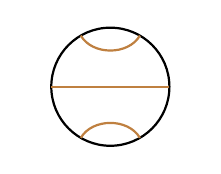
\begin{tikzpicture}[baseline=-0.65ex,scale=0.15]
            \useasboundingbox (-7, -5) rectangle (7, 5);
            \draw[thick] (-0, 0) circle (5);
            \draw[thick, brown] (0:5) to (180:5);
            \draw[thick, brown] (60:5) [in=-60,out=-120] to (120:5);
            \draw[thick, brown] (-60:5) [in=60,out=120] to (-120:5);
        \end{tikzpicture}$
        \subcaption{}
    \end{minipage}
    \begin{minipage}[b]{.18\linewidth}
        \centering
        $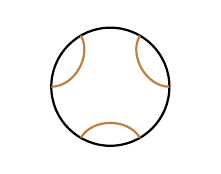
\begin{tikzpicture}[baseline=-0.65ex,scale=0.15]
            \useasboundingbox (-7, -5) rectangle (7, 5);
            \draw[thick] (-0, 0) circle (5);
            \draw[thick, brown] (0:5) [in=-120, out=180] to (60:5);
            \draw[thick, brown] (120:5) [in=0, out=-60] to (180:5);
            \draw[thick, brown] (240:5) [in=120, out=60] to (300:5);
        \end{tikzpicture}$
        \subcaption{}
    \end{minipage}
    \begin{minipage}[b]{.18\linewidth}
        \centering
        $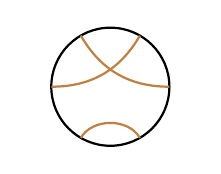
\begin{tikzpicture}[baseline=-0.65ex,scale=0.15]
            \useasboundingbox (-7, -5) rectangle (7, 5);
            \draw[thick] (-0, 0) circle (5);
            \draw[thick, brown] (0:5) [out=180, in=-60] to (120:5);
            \draw[thick, brown] (60:5) [in=0,out=-120] to (180:5);
            \draw[thick, brown] (240:5) [in=120, out=60] to (300:5);
        \end{tikzpicture}$
        \subcaption{}
    \end{minipage}
    \begin{minipage}[b]{.18\linewidth}
        \centering
        $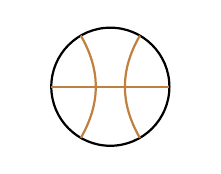
\begin{tikzpicture}[baseline=-0.65ex,scale=0.15]
            \useasboundingbox (-7, -5) rectangle (7, 5);
            \draw[thick] (-0, 0) circle (5);
            \draw[thick, brown] (0:5) to (180:5);
            \draw[thick, brown] (60:5) [in=120,out=-120] to (300:5);
            \draw[thick, brown] (120:5) [in=60, out=-60] to (240:5);
        \end{tikzpicture}$
        \subcaption{}
    \end{minipage}
    \begin{minipage}[b]{.18\linewidth}
        \centering
        $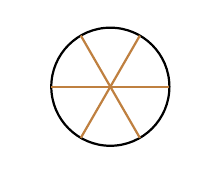
\begin{tikzpicture}[baseline=-0.65ex,scale=0.15]
            \useasboundingbox (-7, -5) rectangle (7, 5);
            \draw[thick] (-0, 0) circle (5);
            \draw[thick, brown] (0:5) to (180:5);
            \draw[thick, brown] (60:5) to (240:5);
            \draw[thick, brown] (120:5) to (300:5);
        \end{tikzpicture}$
        \subcaption{}
    \end{minipage}
    \caption{Wszystkie pięć diagramów cięciw stopnia 3}
\end{figure}
\end{comment}

\begin{tobedone}
    Jak zamienić węzeł w diagram cięciw?
\end{tobedone}

\begin{proposition}
    Niech $K_1, K_2$ będą dwoma singularnymi węzłami o~tym samym diagramie cięciw, zaś $v$~niezmiennikiem Wasiljewa.
    Wtedy $v(K_1) = v(K_2)$.
\end{proposition}

\begin{proof}
    Umieśćmy węzły singularne $K_1, K_2$ w przestrzeni tak, by ich wierzchołki oraz obie gałęzie wychodzące z wierzchołków leżały tak samo. Wtedy można tak zdeformować łuki $K_1$ tak, by jedynymi osobliwościami, jakie się pojawią lub znikną, były podwójne punkty.
    Teraz kłębiasta Wasiljewa mówi, że wartość $v$ nie zmienia się podczas tego procesu, zatem $v(K_1) = v(K_2)$, co należało okazać.
    % chmutov12
    % TODO: (\cite{duzhin12}, prop. 3.4.2)
\end{proof}

\begin{definition}[symbol niezmiennika]
    Niech $v$ będzie niezmiennikiem Wasiljewa.
    Obcięcie $v$ do zbioru węzłów singularnych o~dokładnie $n$ wierzchołkach traktowane jako funkcja ze zbioru diagramów cięciw nazywamy symbolem tego niezmiennika.
\end{definition}

Jeśli $v_1, v_2$ są niezmiennikami Wasiljewa rzędu co najwyżej $n$ o~tych samych symbolach, to ich różnica jest niezmiennikiem rzędu co najwyżej $n - 1$.
Oznacza to, że przestrzeń $\mathcal V_n/\mathcal V_{n-1}$ pokrywa się z przestrzenią wszystkich symboli niezmienników Wasiljewa rzędu co najwyżej $n$.
Zbiór diagramów cięciw rzędu $n$ jest skończony, więc przestrzeń funkcji na tym zbiorze też jest skończona, a zatem przestrzenie $\mathcal V_n$ są skończonego wymiaru.

Symbol nie jest byle jaką funkcją, spełnia dwie relacje:

\begin{comment}
\begin{figure}[H]
$$
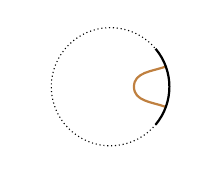
\begin{tikzpicture}[baseline=-0.65ex,scale=0.15]
    \useasboundingbox (-7, -5) rectangle (7, 5);
    \draw[densely dotted] (-0, 0) circle (5);
    \draw[thick, brown] (20*17:5) [out=180+17*20, in=down] to (0:2) [in=180+1*20, out=up] to (20*1:5);
    \draw[thick] (20*16:5) arc (20*16:20*20:5);
\end{tikzpicture}
\mapsto 0
$$
\caption{Relacja ,,one-term'' (1T albo FI?)}
\end{figure}
oraz
\begin{figure}[H]
$$
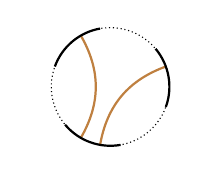
\begin{tikzpicture}[baseline=-0.65ex,scale=0.15]
    \useasboundingbox (-7, -5) rectangle (7, 5);
    \draw[densely dotted] (-0, 0) circle (5);
    \draw[thick, brown] (20*1:5) [in=180+13*20, out=180+1*20] to (20*13:5);
    \draw[thick, brown] (20*6:5) [in=180+12*20, out=180+6*20] to (20*12:5);
    \draw[thick] (20*5 :5) arc (20*5 :20*8 :5);
    \draw[thick] (20*11:5) arc (20*11:20*14:5);
    \draw[thick] (20*17:5) arc (20*17:20*20:5);
\end{tikzpicture}
-
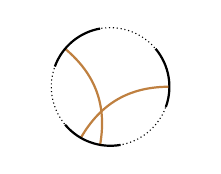
\begin{tikzpicture}[baseline=-0.65ex,scale=0.15]
    \useasboundingbox (-7, -5) rectangle (7, 5);
    \draw[densely dotted] (-0, 0) circle (5);
    \draw[thick, brown] (20*0:5) [in=180+12*20, out=180+0*20] to (20*12:5);
    \draw[thick, brown] (20*7:5) [in=180+13*20, out=180+7*20] to (20*13:5);
    \draw[thick] (20*5 :5) arc (20*5 :20*8 :5);
    \draw[thick] (20*11:5) arc (20*11:20*14:5);
    \draw[thick] (20*17:5) arc (20*17:20*20:5);
\end{tikzpicture}
+
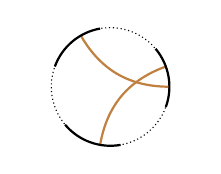
\begin{tikzpicture}[baseline=-0.65ex,scale=0.15]
    \useasboundingbox (-7, -5) rectangle (7, 5);
    \draw[densely dotted] (-0, 0) circle (5);
    \draw[thick, brown] (20*0:5) [in=180+6*20, out=180+0*20] to (20*6:5);
    \draw[thick, brown] (20*1:5) [in=180+13*20, out=180+1*20] to (20*13:5);
    \draw[thick] (20*5 :5) arc (20*5 :20*8 :5);
    \draw[thick] (20*11:5) arc (20*11:20*14:5);
    \draw[thick] (20*17:5) arc (20*17:20*20:5);
\end{tikzpicture}
-
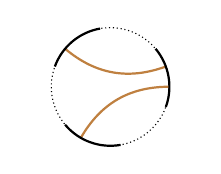
\begin{tikzpicture}[baseline=-0.65ex,scale=0.15]
    \useasboundingbox (-7, -5) rectangle (7, 5);
    \draw[densely dotted] (-0, 0) circle (5);
    \draw[thick, brown] (20*0:5) [in=180+12*20, out=180+0*20] to (20*12:5);
    \draw[thick, brown] (20*1:5) [in=180+7*20, out=180+1*20] to (20*7:5);
    \draw[thick] (20*5 :5) arc (20*5 :20*8 :5);
    \draw[thick] (20*11:5) arc (20*11:20*14:5);
    \draw[thick] (20*17:5) arc (20*17:20*20:5);
\end{tikzpicture}
\mapsto 0.
$$
\caption{Relacja ,,four-term'' (4T)}
\end{figure}
\end{comment}

Diagramy mogą mieć więcej cięciw z końcami tam, gdzie linia jest kropkowana, natomiast wszystkie końce cięciw na czarnych, pogrubionych łukach zostały zaznaczone explicite.

Zastosowaliśmy tutaj mały skrót dla oszczędności miejsca: oczywiście nie umiemy jeszcze odejmować od siebie diagramów, dlatego powyższe relacje należy rozumieć tak, że na każdym diagramie liczymy symbol niezmiennika i porównujemy tak otrzymane liczby zespolone.

\begin{definition}[układ ciężarów]
    Funkcję określoną na zbiorze diagramów $n$ cięciw, która spełnia relacje 1T oraz 4T, nazywamy układem ciężarów.
% DICTIONARY;weight system;układ ciężarów
\end{definition}

Okazuje się, że wszystkie zależności, jakie występują między niezmiennikami Wasiljewa, są konsekwencjami relacji 1T oraz 4T.
Mówi o~tym głębokie twierdzenie Koncewicza:

\begin{proposition}
    Każdy układ ciężarów jest symbolem pewnego niezmiennika Wasiljewa. % rzędu co najwyżej $n$ - nie mieści się, przenosi samo $n$ do nowej linii.
\end{proposition}

\begin{proof}
    Koncewicz w \cite{kontsevich93}. % chmutow12/chmutov11 theorem 3.4
\end{proof}

\begin{definition}[chiński znak]
    Spójny graf złożony z pojedynczego zorientowanego okręgu oraz pewnej liczby niezorientowanych, kreskowanych linii, które mogą się spotykać w~jednym z dwóch typów wierzchołków:
    \begin{itemize}
        \item wewnętrznych wierzchołkach, gdzie spotykają się trzy kreskowane linie;
        \item zewnętrznych wierzchołkach, gdzie kreskowane linie kończą się na okręgu.
    \end{itemize}
    Wierzchołki wewnętrzne są zorientowane, zgodnie lub przeciwnie do ruchu wskazówek zegara.
\end{definition}

Diagramy cięciw modulo relacja 4T jest tym samym, co algebra chińskich znaków modulo relacja STU.
\index{algebra!chińskich znaków}%
W~tej drugiej spełnione są jeszcze relacje AS oraz IHX, nie mam siły tego rysować, ale wszystko można znaleźć w pracy Bar-Natana \cite{barnatan_95}.

\begin{tobedone}
    % DICTIONARY;actuality table;tablica rzeczywistości
    \index{tablica rzeczywistości?}
    Actuality tables.
\end{tobedone}

Stojmenow w \cite{stoimenow_01} pokazał, że niezmienniki Wasiljewa każdego rzędu można wyznaczyć w~skończonym czasie.
Dokładniej:

\begin{proposition}
    Niezmiennik Wasiljewa rzędu co najwyżej $k$ jest jednoznacznie określony przez wartości, jakie przyjmuje na alternujących węzłach o co najwyżej $2k^2 + k$ skrzyżowaniach.
\end{proposition}

Oczywiście wynik ten onie ma to żadnego praktycznego zdarzenia, ponieważ już dla $k = 4$ musielibyśmy znać wszystkie węzły o 36 skrzyżowaniach (a~jeszcze ich nie znamy, stan na 2021 rok).

Niezmienniki Wasiljewa nie są zupełne.
Ohyama dla każdego węzła $K$ i~liczby naturalnej $n$ wskazał jawnie nieskończoną rodzinę złożonych węzłów, których niezmienniki rzędu co najwyżej $n$ nie odróżniają od $K$ (\cite{ohyama95}).
Stanford rozszerzył ten wynik: w~\cite{stanford96} udowodnił, że dla każdego splotu $L$ istnieje nieskończona rodzina pierwszych, nierozszczepialnych, alternujących splotów nieodróżnialnych takimi niezmiennikami.

Z drugiej strony, Chmutow i inni piszą w \cite{duzhin12}, że sześć niezmienników rzędu co najwyżej 4 wystarcza do odróżnienia dowolnych dwóch węzłów pierwszych do 8 skrzyżowań.
Kneissler twierdzi (\cite[wniosek 2.5]{kneissler97}), że niezmienniki rzędu co najwyżej 12 nie odróżniają węzłów od ich odwrotności.
\index{węzeł!odwrotny}%

W 1993 roku Maxim Koncewicz pokazał, że dla każdego węzła można policzyć pewną całkę (teraz nazywaną całką Koncewicza), która jest uniwersalnym niezmiennikiem Wasiljewa.
\index{całka Koncewicza}
Oznacza to, że z jej wartości można odtworzyć wszystkie inne niezmienniki skończonego typu.
Bar-Natan w 1995 roku znalazł wartość tej całki dla niewęzła:
\begin{equation}
    I (\LittleUnknot) = \exp \left(\sum_{n=0}^\infty b_{2n} w_{2n}\right),
\end{equation}
gdzie $b_{2n}$ to zmodyfikowane liczby Bernoulliego o funkcji tworzącej
\begin{equation}
    \sum_{n=0}^\infty b_{2n} x^{2n} = \frac 12 \log \frac {e^{x/2} - e^{-x/2}}{x/2},
\end{equation}
zaś $w_{2n}$ to ,,koła'': diagramy okręgu z doczepionymi $2n$ promieniami.
Liniową kombinację należy rozumieć jako element algebry chińskich znaków.
\index{algebra!chińskich znaków}%
Następnie Marché w~2003 roku znalazł wartości całki dla węzłów torusowych (\cite{marche04}).
Wygląda na to, że nikt nie odważył się dokonać tego dla innych węzłów (stan na 2019).

\begin{conjecture}
    \label{con:vassilliev}
    Uniwersalny niezmiennik Wasiljewa jest zupełny.
\end{conjecture}

Całka Koncewicza jest mocniejsza od każdego wielomianowego niezmiennika, jaki dotąd poznaliśmy.
Wynika stąd, że stanowić będzie dużo trudniejszy problem niż dowód hipotezy \ref{con:jones} mówiącej, że wielomian Jonesa wykrywa niewęzły.

% DICTIONARY;link, string;splot, sznurkowy
Chmutow, Dużin wspominają w bardzo czytelnie napisanym artykule \cite{chmutov05}, że hipoteza \ref{con:vassilliev} jest prawdziwa dla splotów sznurkowych i warkoczy, jak dowiedziono w \cite{kohno87}, \cite{barnatandror95}.
\index{splot!sznurkowy}%
\index{warkocz}%

\index{niezmiennik!Wasiljewa|)}

% koniec sekcji niezmienniki Wasiljewa
